\documentclass{article}

\usepackage[margin=2.5cm,left=2cm,includefoot]{geometry}
\usepackage{graphicx}
\usepackage{float}
\usepackage[space]{grffile}
\usepackage{hyperref}
\usepackage[export]{adjustbox}
\usepackage{multicol}
\usepackage{caption}
\usepackage{hyperref}
\usepackage{listings}
\usepackage{vhistory}
\usepackage{titlesec}

\setcounter{secnumdepth}{4}

\titleformat{\paragraph}
{\normalfont\normalsize\bfseries}{\theparagraph}{1em}{}
\titlespacing*{\paragraph}
{0pt}{3.25ex plus 1ex minus .2ex}{1.5ex plus .2ex}

% Header and footer
\usepackage{fancyhdr}
\pagestyle{fancy}

\rhead{COS301}
\lhead{Testing Document}
\fancyfoot[R]{Page \thepage}

\renewcommand{\headrulewidth}{2pt}
\renewcommand{\footrulewidth}{1pt}

\begin{document}

	\begin{titlepage}
		\begin{center}
			
\includegraphics[width=10cm]{images/UP.jpg}  \\
			[0.5cm]
			\huge{
			Test Plan and Report\\
			}
			
			\line(1,0){300}\\
			[0.2cm]
			\LARGE{MarketLead.io\\
			Client: RetroRabbit} \\
			\line(1,0){300}\\
			\LARGE{Team: Valknut Solutions}\\
			[1.0cm]
			\large{Version: 1.3}\\
			[1.0cm]
			\large
			{
			\begin{itemize}
				\item 13054903 - Charl Jansen van Vuuren    
				\item 13044924 - Kevin Heritage
				\item 13176545 - Quinton Weenink\\
			\end{itemize}
			}
			\textsc{\large}\\
		[3.0cm]
		\textsc{\large  Department of Computer Science}\\
		[0.5cm]
		\textsc{\large \today}\\
		\end{center}
	\end{titlepage}
	
	\cleardoublepage
	% Start of the revision history table
	\begin{versionhistory}
  		\vhEntry{1.0}{27.7.2016}{CJvV,KH,QW}{created}
  		\vhEntry{1.1}{04.9.2016}{CJvV,KH,QW}{Updated format based on template on CS web, added new test information}
  		\vhEntry{1.2}{27.9.2016}{CJvV,KH,QW}{Added to conclusion, testing in general and test summary, updated heading to new product name}
  		\vhEntry{1.3}{30.9.2016}{CJvV,KH,QW}{Added Facebook messenger unit tests, updated testing tables, added detailed overview of new tests, updated paths to tests}
	\end{versionhistory}	
	
	\cleardoublepage
	\tableofcontents
	\cleardoublepage
	
\section{Introduction}
This document contains information related to Testing of the Insurance Profiling project that is being developed for RetroRabbit as part of the COS301 module at the University Of Pretoria. \\
This document is based on the IEEE 829 Standard for Testing Documentation \href{http://www.fit.vutbr.cz/study/courses/ITS/public/ieee829.html}{IEEE 829}
The structure of this document includes an initial scope and purpose, a Unit test plan and the final Unit test report.
\subsection{Purpose}
This document combines the unit test plan and report into a single coherent artefact. The overall purpose of the system is to allow the analysis of different social media inputs (Facebook in particular) by means of a marketing and risk analysis standpoint.
Test driven development is crucial to our system as it ensures every added feature is compatible with the current version of the system and that feature is working as intended.
\subsection{Scope}
The scope of this document is structured as follows. The features that are considered for testing are listed as per section \ref{sec:testItems}. \\
Tests that have been identified from the requirements are
discussed in detail in section \ref{sec:FeaturesTest}.\\
Furthermore, this document outlines the test environment and the risks involved in the testing approaches that will be followed as per section \ref{subsec:testEnvironment}. Assumptions and dependencies of this test plan will also be mentioned as per section \ref{subsec:assumptions} . Section \ref{sec:FeaturesTest} , \ref{sec:testCases} and \ref{sec:testReport} outlines, discusses and concludes on the results of the tests, respectively.
\subsection{Test Environment}\label{subsec:testEnvironment}
The testing environment is mainly software based and includes:
\begin{itemize}
	\item Programming languages:
	\begin{itemize}
		\item Javascript 
	\end{itemize}
	\item Testing Frameworks:
	\begin{itemize}
		\item MochaJS - Unit tests
		\item Travis CI - Continuous integration for deployment
	\end{itemize}
	\item Coding Environment:
	\begin{itemize}
		\item NodeJS based web server
		\item ExpressJS
		\item PostgreSQL database with Sequelize ORM
		\item Terminal based test outputs
	\end{itemize}
	\item Operating system:
	\begin{itemize}
		\item Ubuntu Linux
		\item Microsoft Windows 10
	\end{itemize}
	\item Internet Browsers:
	\begin{itemize}
		\item Mozilla Firefox
		\item Chrome web browser
	\end{itemize}
\end{itemize}

\subsection{Assumptions and Dependencies}\label{subsec:assumptions}
Assumptions:
\begin{itemize}
	\item An instance of the server is running locally(for Unit tests)
	\item External server is active (for Deploy tests only)
	\item Active internet connection (for Deploy tests only)
	\item NodeJS and Node package manager is installed works as intended
	\item Mocha is installed and works as intended
\end{itemize}
Dependencies:
\begin{itemize}
	\item Travis CI 
	\item Mocha framework
	\item Chai (part of Mocha)
	\item Heroku platform as a service (Integration tests)
	\item Assert package from npm
	\item fbController.js test file
	\item graphTest.js test file
	\item test.js test file
\end{itemize}


\section{Test items}\label{sec:testItems}
\subsection{The items included in this test document:}
\begin{itemize}
	\item Backend API calls
	\item Functional unit tests
	\item Database management functions
	\item Environmental tests 
	\item Deployment and compatibility tests
\end{itemize} 

\pagebreak
\section{Functional Features to be Tested}\label{sec:FeaturesTest}
\paragraph{Test estimation can be categorized as fast (nearly instant tests) or slow (timely tests with external dependencies) for our system.} 
\subsection{Overall approach with regards to adequate testing of :} 
\begin{itemize}
\item Feature unit tests:
\begin{itemize}
	\item Mocking out the non essential dependencies to be able to test the feature
	\item Include the essential dependencies that cannot be mocked out
	\item Estimation of this feature group can be concluded as "fast".
\end{itemize}
\item Backend API tests:
\begin{itemize}
	\item Estimation of this feature group can be concluded as "slow" as it is dependent on the external server.
\end{itemize}
\item Environmental tests:
\begin{itemize}
	\item Estimation of this feature group can be concluded as "fast" as it is a simple check for current environment.
\end{itemize}
\item Deployment tests:
\begin{itemize}
	\item Estimation of this feature group can be concluded as "slow" as it is dependent on the external Travis CI server.
\end{itemize}
\end{itemize}

\subsection{The included features to be tested:}
\begin{itemize}
\item Feature unit tests:
	\begin{itemize}
	\item The ability to receive data from a Facebook lead ad and save this data in the database.
	\item The ability to receive data from any other integration point as per the specified format.
	\item The ability to receive data from the Facebook messenger integration point.
	\item These feature relates to the getLeadData use case in the Functional requirements documentation
	\item The calculation of Age from a datestring object
	\item The calculation of Months from a datestring object
	\end{itemize}
	
\item API calls to do:
	\begin{itemize}
	\item Database insertions 
	\item Database deletions 
	\item Database retrievals 
	\item This test relates to the Analysis use case in the Functional requirements documentation, it forms the underlying persistence with regards to the data analysis is done on.
	\end{itemize}
\item Environmental test
	\begin{itemize}
	\item Integration test to determine the current environment (development or deployment) to react accordingly 
	\end{itemize}
\item Deployment/Build testing including Compatibility
		\begin{itemize}
	\item Automated testing by the Travis CI framework to ensure the current feature is compatible with different versions of the NodeJS framework. 
	\end{itemize}
\end{itemize}

\begin{table}[H]
\centering
\caption{Test cases}
\label{test_table}
\begin{tabular}{|l|l|l|l|}
\hline
Feature ID & RDS Source                            & Summary                                    & Test Case ID \\ \hline \hline
1          & Functional requirements - getLeadData & Receive data from a Facebook lead ad       & 1            \\ \hline
2          & Functional requirements - getData     & Receive data from other integration source & 2            \\ \hline
3          & Functional requirements - Analysis    & Database insertions                        & 3            \\ \hline
4          & Functional requirements - Analysis    & Database deletions                         & 4            \\ \hline
5          & Functional requirements - Analysis    & Database retrievals                        & 5            \\ \hline
6          & Functional requirements - generateReport & Extract age from datestring			    & 6			   \\ \hline
7	       & Functional requirements - generateReport & Extract month from datestring			& 7            \\ \hline
8          &  Architecture design - Section 5      & Environmental test                         & 8            \\ \hline
9          &  Architecture design - Section 5.1.1  & Deployment test                            & 9            \\ \hline
10         &  Functional requirements - getMessengderData & Receive data from a Facebook messenger & 10            \\ \hline
\end{tabular}
\end{table}


\section{Test instructions} 
\begin{itemize}
\item Unit Tests can be run with the command "npm test" which will run Mocha.
\item API tests can be run with the command "npm run-script apitest"
\item Integration tests can be run with the command "npm run-script integrationtest".  
\item If these tests are ran locally they will connect to the local database.
\item Travis CI runs these test to the external database hosted on Heroku. The Travis tests are ran when a new branch is merged to ensure compatibility with all versions of Node.
\end{itemize}
\cleardoublepage
\section{Test cases}\label{sec:testCases}
\subsection{\underline{Test Case 1: getLeadData}}\label{test1}
\subsubsection{Condition 1: Ad is submitted with all valid fields }
\paragraph{Objective:} The purpose of this test is to extract data from a filled in Facebook lead ad and save this data if valid.
\paragraph{Input:} The following inputs will be used:
\begin{enumerate}
	\item An non-existing entity - based on Facebook user data:
	\begin{enumerate}
		\item firstName
  		\item lastName
  		\item mobileNumber 
  		\item maritalStatus 
  		\item dateOfBirth 
 		\item gender
  		\item location 
 		\item email	
	\end{enumerate}
\end{enumerate}
\paragraph{Outcome:} The following outcomes are expected for a pass result:
\begin{enumerate}
	\item A JSON object of a User passed to the Condition 3
\end{enumerate}
\subsubsection{Condition 2: Invalid inputs}
\paragraph{Objective:} The purpose of this test is to return an empty user if the inputs are not valid
\paragraph{Input:} The following inputs will be used:
\begin{enumerate}
	\item A unpopulated user object
\end{enumerate}
\paragraph{Outcome:} The following outcomes are expected for a pass result:
\begin{enumerate}
	\item Returns an empty user
\end{enumerate}
\subsubsection{Condition 3: Valid data inputs}
\paragraph{Objective:} The purpose of this test is to return a valid JSON object of the data for saving purposes.
\paragraph{Input:} The following inputs will be used:
\begin{enumerate}
	\item An existing object of User as per Condition 1
\end{enumerate}
\paragraph{Outcome:} The following outcomes are expected for a pass result:
\begin{enumerate}
	\item A new User passed to the database
\end{enumerate}

\subsection{\underline{Test Case 2: getData}}\label{test2}
\subsubsection{Condition 1: Valid inputs }
\paragraph{Objective:} The purpose of this test is to extract data from any integration source.
\paragraph{Input:} The following inputs will be used:
\begin{enumerate}
	\item An non-existing entity - based on user data from any integration:
	\begin{enumerate}
		\item firstName
  		\item lastName
  		\item mobileNumber 
  		\item maritalStatus 
  		\item dateOfBirth 
 		\item gender
  		\item location 
 		\item email	
	\end{enumerate}
\end{enumerate}
\paragraph{Outcome:} The following outcomes are expected for a pass result:
\begin{enumerate}
	\item A JSON object of a User 
\end{enumerate}

\subsection{\underline{Test Case 3: Insertion}}\label{test3}
\subsubsection{Condition 1: Valid inputs }
\paragraph{Objective:} The purpose of this test is to test insertion of data into database.
\paragraph{Input:} The following inputs will be used:
\begin{enumerate}
	\item An existing entity of User object
\end{enumerate}
\paragraph{Outcome:} The following outcomes are expected for a pass result:
\begin{enumerate}
	\item The data will be saved into the database
\end{enumerate}

\subsection{\underline{Test Case 4: Deletion}}\label{test4}
\subsubsection{Condition 1: Valid field to remove }
\paragraph{Objective:} The purpose of this test is to test deletion of data in the database
\paragraph{Input:} The following inputs will be used:
\begin{enumerate}
	\item An existing entity of User in the database
\end{enumerate}
\paragraph{Outcome:} The following outcomes are expected for a pass result:
\begin{enumerate}
	\item The existing entity gets deleted from the database 
\end{enumerate}

\subsection{\underline{Test Case 5: Retrieval}}\label{test5}
\subsubsection{Condition 1: If field exists }
\paragraph{Objective:} The purpose of this test is to test retrieval of data from the database.
\paragraph{Input:} The following inputs will be used:
\begin{enumerate}
	\item An existing entity
\end{enumerate}
\paragraph{Outcome:} The following outcomes are expected for a pass result:
\begin{enumerate}
	\item The existing entity gets returned from the database
\end{enumerate}
\subsubsection{Condition 2: If field does not exists }
\paragraph{Objective:} The purpose of this test is to test retrieval of data from the database.
\paragraph{Input:} The following inputs will be used:
\begin{enumerate}
	\item A non existing entity 
\end{enumerate}
\paragraph{Outcome:} The following outcomes are expected for a pass result:
\begin{enumerate}
	\item The test will return null
\end{enumerate}

\subsection{\underline{Test Case 6: Extract age from datestring}}\label{test6}
\subsubsection{Condition 1: Valid datestring object }
\paragraph{Objective:} The purpose of this test is to retrieve a valid age from a datestring.
\paragraph{Input:} The following inputs will be used:
\begin{enumerate}
	\item "1994-06-05T22:00:00.000Z"
\end{enumerate}
\paragraph{Outcome:} The following outcomes are expected for a pass result:
\begin{enumerate}
	\item A valid age will be returned
\end{enumerate}
\subsubsection{Condition 2: Correct age is returned  }
\paragraph{Objective:}  The purpose of this test is calculate the age from a datestring in the format "1994-06-05T22:00:00.000Z".
\paragraph{Input:} The following inputs will be used:
\begin{enumerate}
	\item "1994-06-05T22:00:00.000Z"
\end{enumerate}
\paragraph{Outcome:} The following outcomes are expected for a pass result:
\begin{enumerate}
	\item The age of 22 is returned as a valid outcome
\end{enumerate}
\subsubsection{Condition 3: Correct age is returned  }
\paragraph{Objective:}  The purpose of this test is calculate the age from a datestring in the format "1998-06-05T22:00:00.000Z".
\paragraph{Input:} The following inputs will be used:
\begin{enumerate}
	\item "1998-06-05T22:00:00.000Z"
\end{enumerate}
\paragraph{Outcome:} The following outcomes are expected for a pass result:
\begin{enumerate}
	\item The age of 18 is returned as a valid outcome
\end{enumerate}


\subsection{\underline{Test Case 7: Extract month from datestring as named month}}\label{test7}
\subsubsection{Condition 1: Valid datestring object }
\paragraph{Objective:} The purpose of this test is to retrieve a valid month from a datestring.
\paragraph{Input:} The following inputs will be used:
\begin{enumerate}
	\item "1994-09-05T22:00:00.000Z"
\end{enumerate}
\paragraph{Outcome:} The following outcomes are expected for a pass result:
\begin{enumerate}
	\item A valid month will be returned as a named month
\end{enumerate}
\subsubsection{Condition 2: Correct age is returned  }
\paragraph{Objective:}  The purpose of this test is calculate the month from a datestring in the format "1994-06-05T22:00:00.000Z".
\paragraph{Input:} The following inputs will be used:
\begin{enumerate}
	\item "1994-06-05T22:00:00.000Z"
\end{enumerate}
\paragraph{Outcome:} The following outcomes are expected for a pass result:
\begin{enumerate}
	\item The string of the month of June is returned
\end{enumerate}
\subsubsection{Condition 3: Correct age is returned  }
\paragraph{Objective:}  The purpose of this test is calculate the month from a datestring in the format "1998-09-05T22:00:00.000Z".
\paragraph{Input:} The following inputs will be used:
\begin{enumerate}
	\item "1998-09-05T22:00:00.000Z"
\end{enumerate}
\paragraph{Outcome:} The following outcomes are expected for a pass result:
\begin{enumerate}
	\item The string of the month of September is returned
\end{enumerate}


\subsection{\underline{Test Case 8: Environmental test(Integration test)}}\label{test8}
\subsubsection{Condition 1: If environment is set to Deployment }
\paragraph{Objective:} The purpose of this test is to set the Environment variable based on the current state of the system, Deployment in this case.
\paragraph{Input:} The following inputs will be used:
\begin{enumerate}
	\item Environment set to deployment
\end{enumerate}
\paragraph{Outcome:} The following outcomes are expected for a pass result:
\begin{enumerate}
	\item Set the hosting port to 80
\end{enumerate}
\subsubsection{Condition 2: If environment is set to Development }
\paragraph{Objective:} The purpose of this test is to set the Environment variable based on the current state of the system, Development in this case.
\paragraph{Input:} The following inputs will be used:
\begin{enumerate}
	\item Environment set to development
\end{enumerate}
\paragraph{Outcome:} The following outcomes are expected for a pass result:
\begin{enumerate}
	\item Set the hosting port to 3000 to avoid conflicts
\end{enumerate}

\subsection{\underline{Test Case 9: Travis CI Deployment test (Integration test) }}\label{test9}
\subsubsection{Condition 1: If hosting version is compatible}
\paragraph{Objective:} The purpose of this test is to ensure the current deployed version is compatible with the external hosting service. This includes dependency versions.
\paragraph{Input:} The following inputs will be used:
\begin{enumerate}
	\item A valid NodeJS and NPM version is used
	\item Mocha tests pass
\end{enumerate}
\paragraph{Outcome:} The following outcomes are expected for a pass result:
\begin{enumerate}
	\item The build will pass
\end{enumerate}
\subsubsection{Condition 2: If hosting version is incompatible}
\paragraph{Objective:} The purpose of this test is to ensure the current deployed version is compatible with the external hosting service. This includes dependency versions.
\paragraph{Input:} The following inputs will be used:
\begin{enumerate}
	\item An unsupported version of NodeJS or NPM is used
	\item Mocha Tests fails
\end{enumerate}
\paragraph{Outcome:} The following outcomes are expected for a pass result:
\begin{enumerate}
	\item The build will error/fail
\end{enumerate}


\subsection{\underline{Test Case 10: Facebook messenger test}}\label{test10}
\subsubsection{Condition 1: Valid user message}
\paragraph{Objective:} The purpose of this test is to ensure the Facebook messenger integration data is extracted from the user message.
\paragraph{Input:} The following inputs will be used:
\begin{enumerate}
	\item An empty user to be populated
	\begin{itemize}
  	\item messageId = 0
    \item firstname = ''
    \item lastname : ''
    \item phonenumber : ''
    \item maritalstatus : ''
    \item dateofbirth : ''
    \item gender : ''
    \item city : ''
    \item email : ''
    \end{itemize}	  
\end{enumerate}
\paragraph{Outcome:} The following outcomes are expected for a pass result:
\begin{enumerate}
	\item A populated user with the values
	\begin{itemize}
  	\item messageId : 1
    \item firstname : 'Quinton'
    \item lastname : 'Weenink'
    \item phonenumber : '071 555 9858'
    \item maritalstatus : 'Married'
    \item dateofbirth : '08/03/1995'
    \item gender : 'male'
    \item city : 'Cape Town'
    \item email : 'fake@gmail.com'
    \end{itemize}	  
\end{enumerate}
\subsubsection{Condition 2: Valid response }
\paragraph{Objective:} The purpose of this test is to ensure the correct response is given for a received message.
\paragraph{Input:} The following inputs will be used:
\begin{enumerate}
	\item A correct response to the given message.
	\begin{itemize}
  	\item messageId : 1
    \item firstname : 'Quinton'
    \item lastname : 'Weenink'
    \item phonenumber : '071 555 9858'
    \item maritalstatus : 'Married'
    \item dateofbirth : '08/03/1995'
    \item gender : 'male'
    \item city : 'Cape Town'
    \item email : 'fake@gmail.com'
    \end{itemize}	  
\end{enumerate}
\paragraph{Outcome:} The following outcomes are expected for a pass result:
\begin{enumerate}
	 \item 8:'You will be contacted shortly...',
     \item 0:'Please reply with your Name:',
     \item 1:'Please reply with your Last name:',
     \item 2:'Please reply with your Phone number:',
     \item 3:'Please reply with your Marital status:',
     \item 4:'Please reply with your Date of birth:',
     \item 5:'Please reply with your Gender:',
     \item 6:'Please reply with your City:',
     \item 7:'Please reply with your Email:'
\end{enumerate}

\pagebreak

\section{Item Pass/Fail criteria}\label{sec:FailPass}
If the specified Pre-conditions are not met the post condition will result as false and the test will fail. \\
If the specified Pre-conditions are met the post-condition will hold true and the test will pass.
\begin{itemize}
\item Extract age from datestring
\begin{itemize}
	\item Condition 1:
	\begin{itemize}
		\item Pre-condition - Valid input datestring object
		\item Post-condition - Valid object is returned
	\end{itemize}
	\item Condition 2 and 3:
	\begin{itemize}
		\item Pre-condition - Valid input datestring object
		\item Post-condition - Correct age is returned
	\end{itemize}

\end{itemize}
\item Extract month from datestring
\begin{itemize}
	\item Condition 1:
	\begin{itemize}
		\item Pre-condition - Valid input datestring object
		\item Post-condition - Valid object is returned
	\end{itemize}
	\item Condition 2 and 3:
	\begin{itemize}
		\item Pre-condition - Valid input datestring object
		\item Post-condition - Correct month is returned
	\end{itemize}

\end{itemize}

\item Creating row in Database
\begin{itemize}
	\item Pre-conditions:
		\begin{itemize}
		\item Database is connected and created
		\item The following values are specified:  
		\begin{itemize}
		\item firstName
  		\item lastName
  		\item mobileNumber 
  		\item maritalStatus 
  		\item dateOfBirth 
 		\item gender
  		\item location 
 		\item email
 		\end{itemize} 
		\end{itemize}
\item Post-condition - The row gets persisted
\end{itemize}
\item Retrieving row in Database
	\begin{itemize}
	\item Pre-condition - The currentUser exists
	\item Post-condition - The currentUser is retrieved 
	\end{itemize}

\item Removing row in Database based on currentUser 
	\begin{itemize}
	\item Pre-condition - The currentUser exists
	\item Post-condition - The currentUser is removed
	\end{itemize}

\item Valid messenger responses for valid inputs
	\begin{itemize}
	\item Pre-condition - The inputs as specified are valid
	\item Post-condition - The output messages are correct based on the inputs.
	\end{itemize}

\item Travis CI build test for Node version 5.11
	\begin{itemize}
	\item Pre-condition - The changes to the branch are compatible with version 5.11
	\item Post-condition - The build will pass successfully 
	\end{itemize}	
	
\item Travis CI build test for Node version 6.2
	\begin{itemize}
	\item Pre-condition - The changes to the branch are compatible with version 6.2
	\item Post-condition - The build will pass successfully 
	\end{itemize}

\end{itemize}


\section{Test Deliverables}
Artefacts to be produced as part of testing include the following:
\begin{itemize}
\item Test Plan Section \ref{sec:testItems} - Section \ref{sec:FailPass}
\item Test Report Section \ref{sec:testReport}
\item Test code \href{https://github.com/QuintonWeenink/ValknutSolutions/tree/develop/test}{Github Link to testing directory}
\end{itemize}
\clearpage
\section{Detailed Test Results}\label{sec:testReport}
\subsection{Overview of Test Results}
All tests were run multiple times to ensure success with the inclusion of the Travis Continuous integration tests to ensure compatibility. Two of the tests failed as a result of the external server not being active at that specific time, these cases form part of integration testing and the normal unit tests make use of mocked out information.\\
The Mocha testing framework was chosen as it integrates well with the Node Package manager system and 
simplifies the creation of writing a new unit test.\\
Travis CI was chosen as integration testing framework to ensure compatibility and deployment capabilities. Travis CI integrates with Github to run tests on all branch merges to ensure compatibility of new features in the main deployment branch.\\
Travis CI runs automated tests per branch merge without the need for developer assistance, this greatly decreases deployment time and ensures compatibility.

\subsection{Functional Requirements Test results}
\begin{table}[H]
\centering
\label{link_table}
\begin{tabular}{|l|l|l|}
\hline
Test ID    & Test Name   & Github Link to File \\ \hline \hline
1          & getLeadData &  \href{https://github.com/QuintonWeenink/ValknutSolutions/blob/develop/test/integration/fbControllerTest.js}{fbControllerTest.js}         \\ \hline
2          & getData  &  \href{https://github.com/QuintonWeenink/ValknutSolutions/blob/develop/test/integration/fbControllerTest.js}{fbControllerTest.js}       \\ \hline
3,4,5      & API tests/Database functions & \href{https://github.com/QuintonWeenink/ValknutSolutions/blob/develop/test/api/test.js}{test.js}         \\ \hline
6          & getAge    & \href{https://github.com/QuintonWeenink/ValknutSolutions/blob/develop/test/graphTest.js}{graphTest.js} \\ \hline
7          & getMonths  & \href{https://github.com/QuintonWeenink/ValknutSolutions/blob/develop/test/graphTest.js}{graphTest.js} \\ \hline 
8          &  Environmental test  & \href{https://github.com/QuintonWeenink/ValknutSolutions/blob/develop/test/test.js}{test.js Line 9-15}\\ \hline
9		   & Compatibility test & \href{https://travis-ci.com/QuintonWeenink/ValknutSolutions/builds/30866212}{Travis CI build nr 130} \\ \hline
10		   & addToUser()/ getMessage() & \href{https://github.com/QuintonWeenink/ValknutSolutions/blob/develop/test/fbMessengerTest.js}{fbMessengerTest.js}   \\ \hline
\end{tabular}
\caption{Links to test files}
\end{table}
\paragraph{All tests are located in the Github repo's testing directory:\href{https://github.com/QuintonWeenink/ValknutSolutions}{Repo}}

\paragraph{The following results were obtained from the tests conducted.}
\subsubsection{Test Case 1 - TC \ref{test1}}
Test case 1 ran with valid inputs.
The data extraction functionality for Facebook works as intended.
\begin{enumerate}
	\item All pre-conditions were met and as a result the post condition remained true
	\item Valid inputs were passed as parameter 
\end{enumerate}
\begin{description}
	\item [Result]: Pass 
\end{description}

\subsubsection{Test Case 2 - TC \ref{test2}}
Test case 2 ran with valid inputs.
The data extraction functionality for any integration works as intended.
\begin{enumerate}
	\item All pre-conditions were met and as a result the post condition remained true
	\item Valid inputs were passed as parameter 
\end{enumerate}

\begin{description}
	\item [Result]: Pass 
\end{description}

\subsubsection{Test Case 3 - TC \ref{test3}}
Test case 3 created a new user in the database.
The API for insertion works as intended.
\begin{enumerate}
	\item All pre-conditions were met and as a result the post condition remained true
	\item Server was live to accept new connections and database functions.
\end{enumerate}

\begin{description}
	\item [Result]: Pass 
\end{description}

\subsubsection{Test Case 4 - TC \ref{test4}}
Test case 4 deleted the new user in the database.
The API for deletion works as intended.
\begin{enumerate}
	\item All pre-conditions were met and as a result the post condition remained true
	\item Server was live to accept new connections and database functions.
\end{enumerate}

\begin{description}
	\item [Result]: Pass 
\end{description}

\subsubsection{Test Case 5 - TC \ref{test5}}
Test case 5 retrieved a user in the database.
The API for retrieval works as intended.
\begin{enumerate}
	\item All pre-conditions were met and as a result the post condition remained true
	\item Server was live to accept new connections and database functions.
\end{enumerate}

\begin{description}
	\item [Result]: Pass 
\end{description}

\subsubsection{Test Case 6 - TC \ref{test6}}
Test case 6 returned the age of 22 and 18. 
The getAge functionality works as intended.
\begin{enumerate}
	\item All pre-conditions were met and as a result the post condition remained true
	\item Correct inputs were passed as parameter 
	\item Correct outputs were returned
\end{enumerate}

\begin{description}
	\item [Result]: Pass 
\end{description}

\subsubsection{Test Case 7 - TC \ref{test7}}
Test case 7 returned the month of June and September. 
The getMonths functionality works as intended.
\begin{enumerate}
	\item All pre-conditions were met and as a result the post condition remained true
	\item Valid inputs were passed as parameter 
	\item Correct inputs were passed as parameter 
	\item Correct outputs were returned
\end{enumerate}

\begin{description}
	\item [Result]: Pass 
\end{description}

\subsubsection{Test Case 8 - TC \ref{test8}}
The local environment is set to development as a result of the environment test.
\begin{enumerate}
	\item Environment returned as development for local
\end{enumerate}

\begin{description}
	\item [Result]: Pass 
\end{description}

\subsubsection{Test Case 9 - TC \ref{test9}}
The build for number 130 passed in Travis CI's log
\begin{enumerate}
	\item The current packages and node version were compatible with the external Heroku server.
	\item The build completed without errors.
\end{enumerate}

\begin{description}
	\item [Result]: Pass 
\end{description}

\subsubsection{Test Case 10 - TC \ref{test10}}
Test case 10 returned a populated user and sent the correct responses based on the inputs.
The Facebook messenger tests work as intended.
\begin{enumerate}
	\item All pre-conditions were met and as a result the post condition remained true
	\item Valid inputs were populated.
	\item Correct inputs were passed as parameter 
	\item Correct messages were returned as outputs.
\end{enumerate}

\begin{description}
	\item [Result]: Pass 
\end{description}


\pagebreak
\section{Other}

	\subsection{Mocha build screenshots}
	
	\begin{figure}[H]
	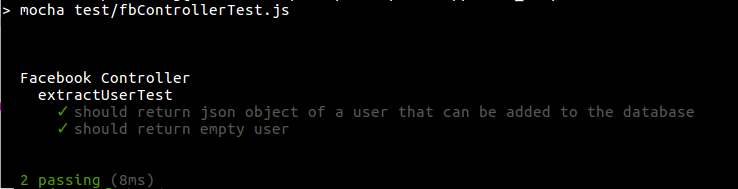
\includegraphics[width=15cm]{images/FbControllerTest.png}
	\caption{getLeadData unit test}
	\end{figure}
	
	\begin{figure}[H]
	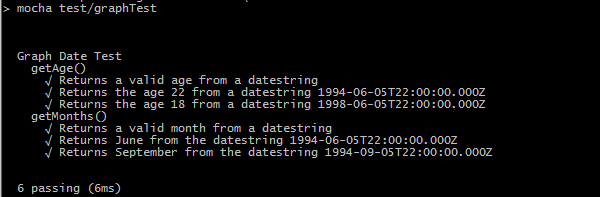
\includegraphics[width=15cm]{images/getAge.png}
	\caption{getAge and getMonth unit test}
	\end{figure}
	
	\begin{figure}[H]
	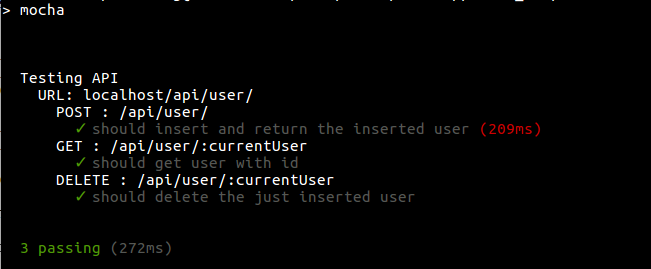
\includegraphics[width=15cm]{images/tests.png}
	\caption{Api Tests}
	\end{figure}
	
	
	\pagebreak
	
	\subsection{Travis build}
	\begin{figure}[H]
	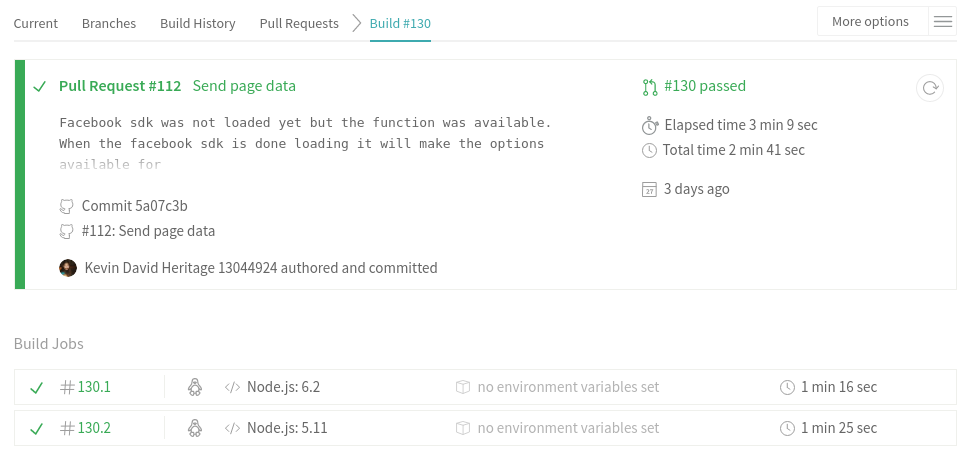
\includegraphics[width=15cm]{images/Travis.png}
	\caption{Travis success }
	\end{figure}	
	
\begin{enumerate}
	\item The mapping of contracts onto tests increases the testability of a system. Mocking out objects eliminates external dependencies which greatly benefit testability. A form of mocking can be seen in Test \ref{test1}
	\item As with the continuous integration model we ensure that the system always stay in a deployable state by means of Travis CI tests and environmental tests. Continuous integration further ensures total compatibility of all new features in each environment (deployment or development).
\end{enumerate}

\pagebreak
\section{Conclusions}
\subsection{General testing conclusions}
\begin{itemize}
\item This project follows a Continous Integration model with regards to testing. Any new feature to be merged with the main branch is first tested, then reviewed by the person merging the branch and only then the merge is closed.

\item  The amount of tests are limited in the current version of the system, this is as a result of the complexity of testing external API calls, such as Facebook, on which our system heavily relies.


\item The ability to modularize functions in NodeJS also complicates the ability to test functionality, this is as a result of the asynchronous callback structure NodeJS uses. 
\item The integration tests will ensure these tests always pass before deploying a new version of the system.
\end{itemize}

\subsection{Test Summary}
\begin{itemize} 
\item All the unit tests completed successfully. Once a test fulfills its pre-condition(s), that test will pass as intended, fulfilling the post-condition. 
\item Test 1 through 10 all passed as intended, as a result of these tests fulfilling their pre-conditions
\end{itemize}
\subsection{Benefits of Testing}
Unit tests in general increases the reliability of a system. Once a new feature is added, that feature must pass its intended tests before even considering integration.\\ \\ This test-driven development method ensures compatibility of new features (integration tests) and that the new feature acts as intended (unit tests). \\
Testing ensures full functionality, reliability and helps other team members understand the added feature. \\ 
The Mocha testing frameworks displays test results a easily understandable way.

\end{document}
